\section{Results and Discussion}
\label{ch1:sec:results-and-discussion}

In this section, all results from the three assessment parts that were outlined in Section \ref{ch1:subsec:method-execution} are presented, and they are briefly discussed, too.
Each assessment focus on improvements in voltage level, power quality, resource utilisation and network losses, in that order.
For completeness and transparency however, the complete analysis of the entire data for each part of the assessment is included in this Thesis' Appendix, Chapter \ref{appx-a:ch1}.

\subsection{Time Series Analysis}
\label{ch1:subsec:time-series-analysis}

The most direct impact on the network's voltage levels would be noticed at the ESMU's PCC.
Therefore, any adjustments to the ESMU's schedule should be most noticeable, too, and its impact can clearly be observed in the figure below.

\begin{figure}\centering
	\subfloat[Voltage levels at ESMU's PCC when minimising its voltage deviation \hl{(nominal substation voltage is 252V)}]{%
		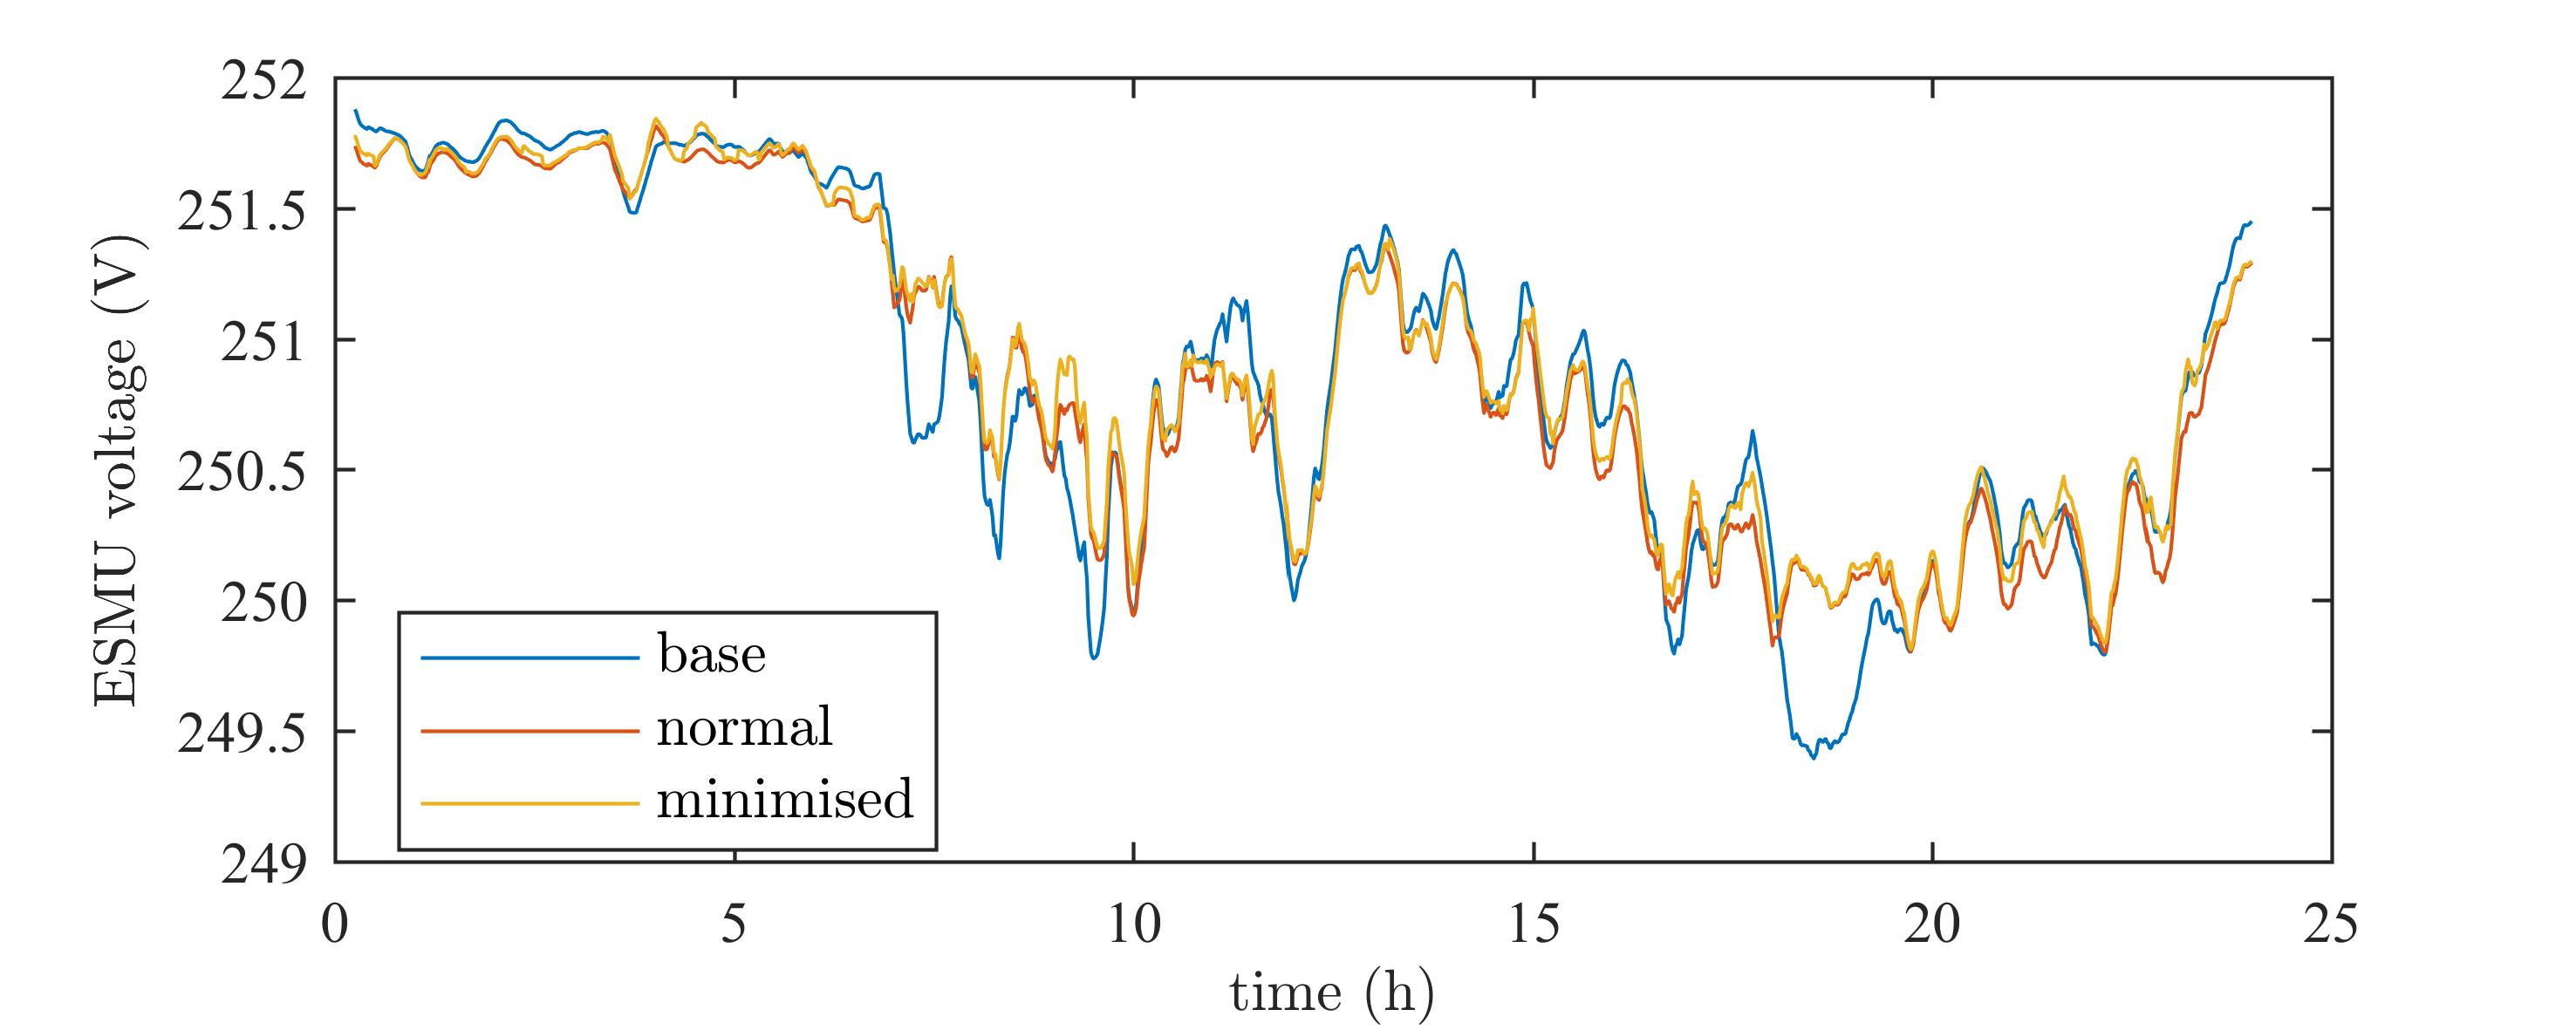
\includegraphics{_chapter1/fig/results/ts-esmu-voltages_}%
		\label{ch1:subfig:ts-esmu-voltage}%
	}\\
%	\vspace{5mm}
	\subfloat[Cost associated with the minimisation of the ESMU's PCC voltage deviation]{%
		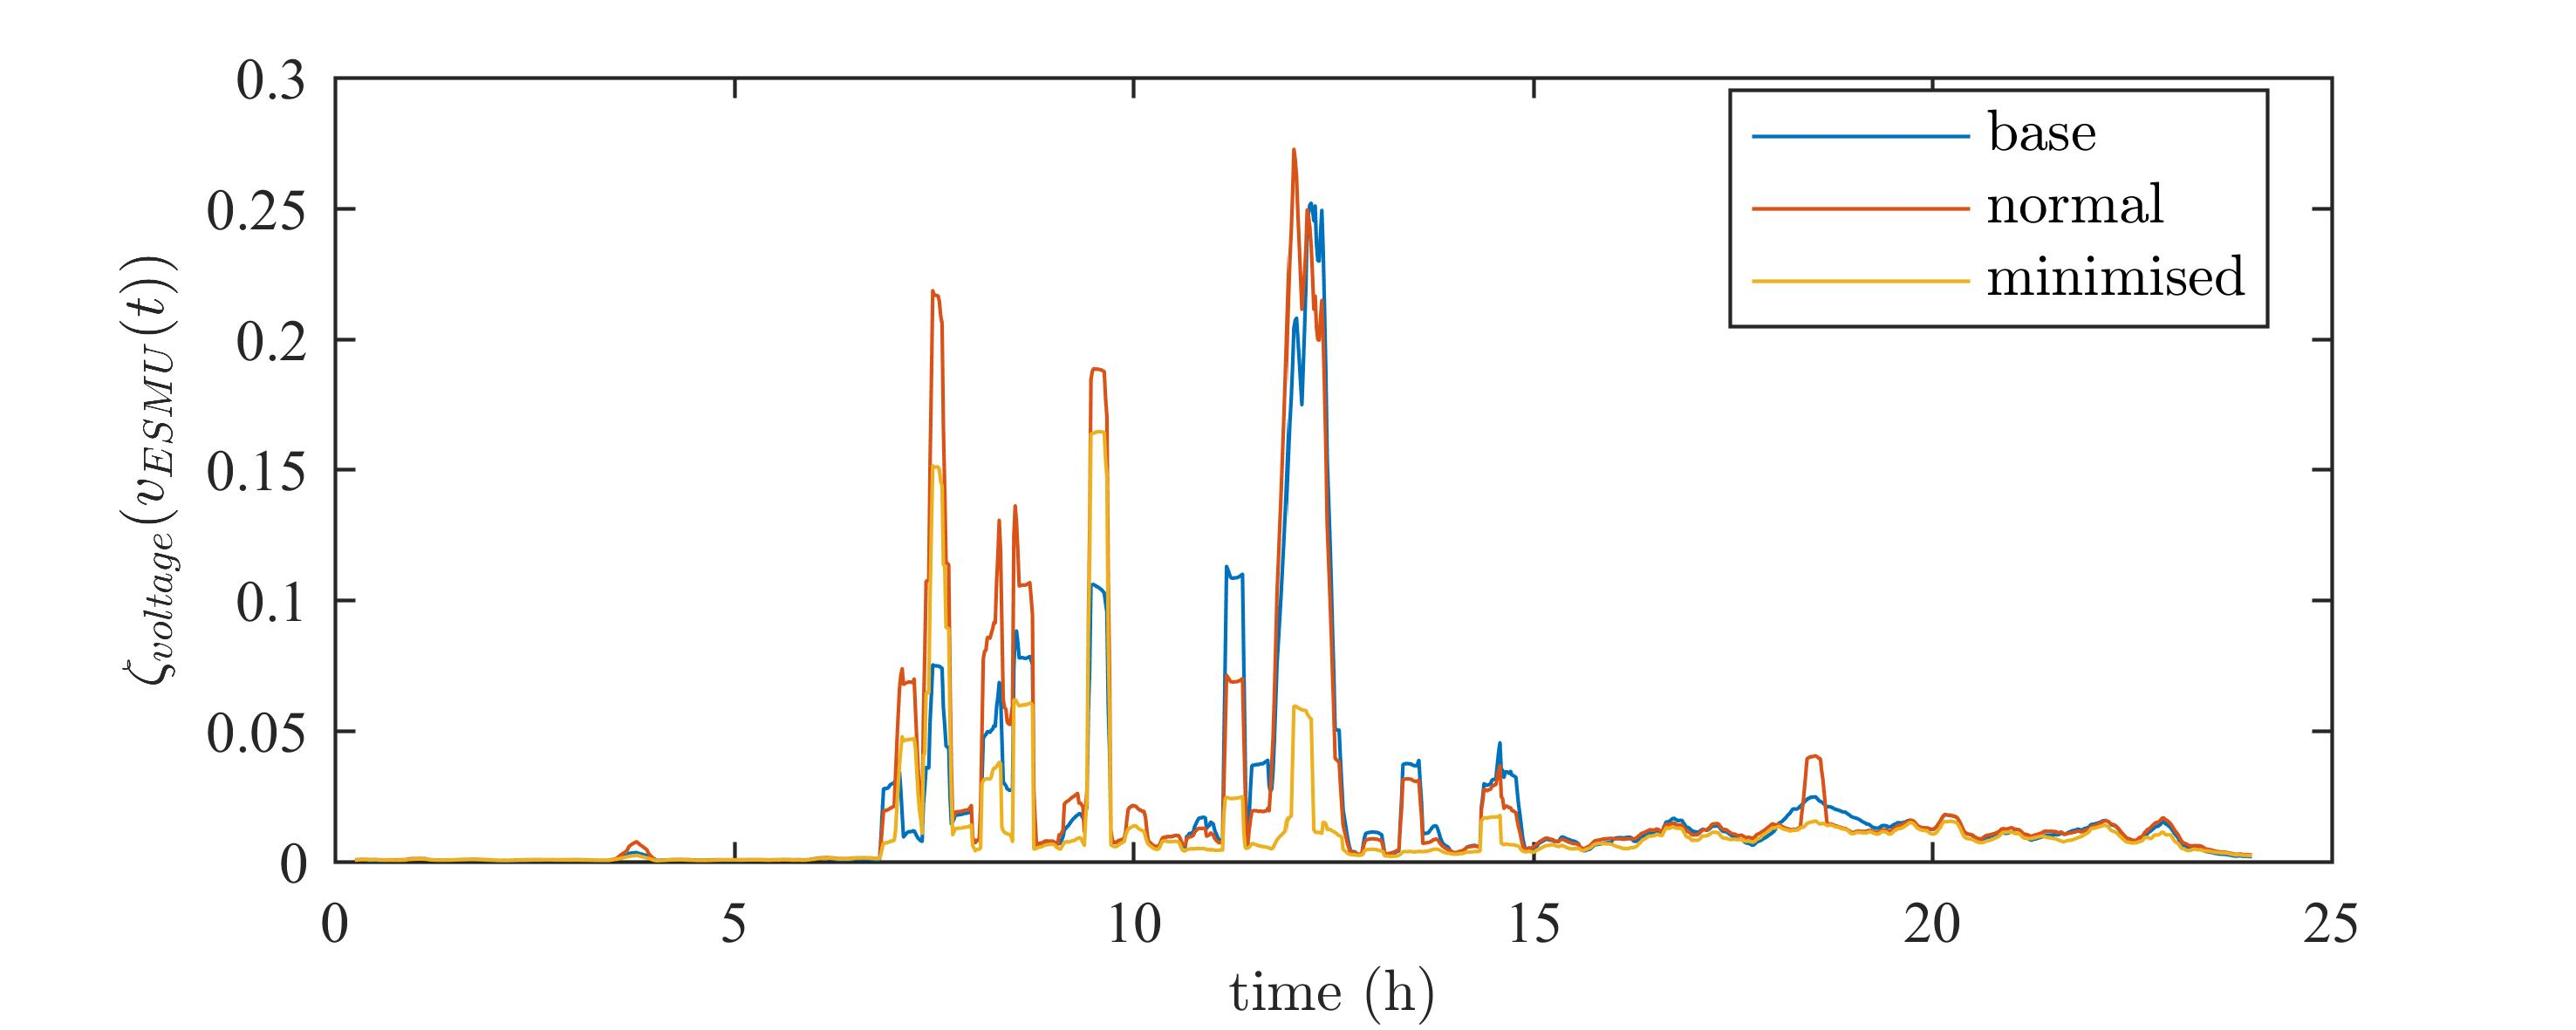
\includegraphics{_chapter1/fig/results/ts-esmu-voltages}%
		\label{ch1:subfig:ts-esmu-voltage-cost}%
	}
\caption{Voltage level modifications as noted at the ESMU's PCC by adjusting its schedule}
\label{ch1:fig:ts-esmu-voltages}
\end{figure}

Here, in Figure \ref{ch1:subfig:ts-esmu-voltage}, the base and normal case's voltage profiles are plotted alongside the case for which the deviation from substation voltage is minimised.
For reference, the nominal substation voltage (i.e. the default IEEE Test Case P2N voltage) has been included for reference.
From this figure it can be observed that during the night's light load (i.e. from 0:00 to 6:00), the ESMU was capable of boosting its voltage towards its nominal feeder voltage.
This is also the case during the lighter afternoon load (i.e. between 12:00-14:00).
Yet during the rest of the day, the ESMU noticeably failed to match its PCC voltage to the network's nominal substation voltage.
The reason behind this behaviour is the fact that the ESMU already reserved its resources to cater for its underlying half-hourly schedule.
Therefore, the remaining resources to provide voltage support become more limited.
Combined with the fact that the LV distribution network is more resistive than inductive (i.e. unlike HV transmission networks), reactive power injection to support voltage levels has a reduced impact.
Nonetheless, due to the constant yet small availability of power resources, the ESMU was able to boost voltages by to some extent at all times; this can be seen in Figure \ref{ch1:subfig:ts-esmu-voltage-cost}, where the associated cost has always been reduced in comparison to the base and normal.

The ability to support voltage levels at the ESMU's PCC is interesting, yet to support voltage levels at all buses throughout the network is more relevant, since some of these buses are linked to customers, for which maintaining a constant voltage level is essential.
Therefore, the next voltage plot inspects both the highest and lowest voltage level that was recorded throughout the network.

\begin{figure}\centering
	\subfloat[Highest and lowest voltage levels that were recorded throughout the network when minimising the worst voltage deviation \hl{(nominal substation voltage is 252V)}]{%
		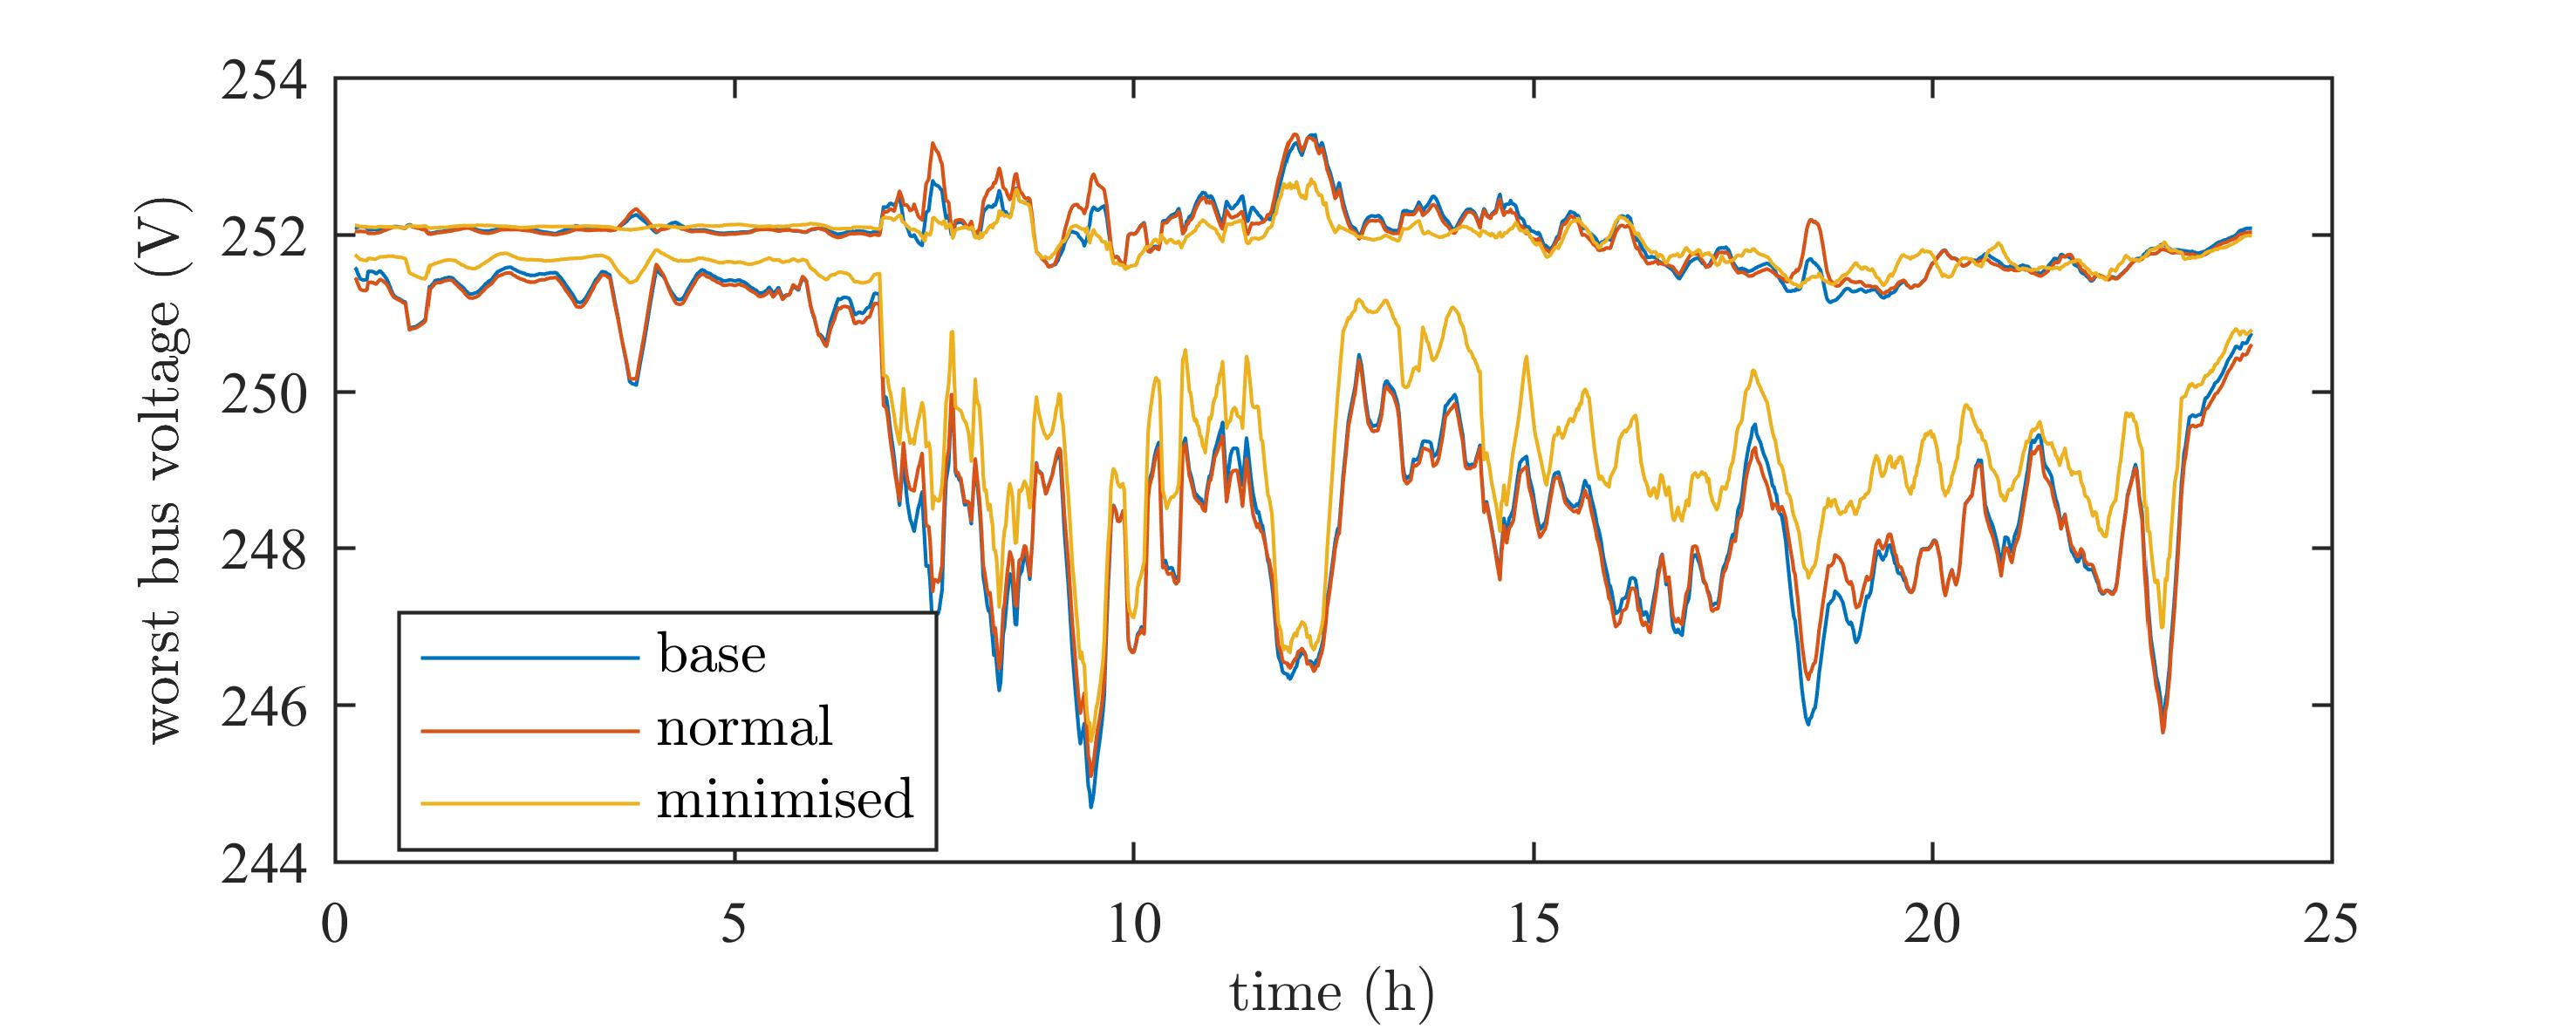
\includegraphics{_chapter1/fig/results/ts-all-voltages_}%
		\label{ch1:subfig:ts-all-voltages}%
	}\\
%	\vspace{5mm}
	\subfloat[Cost associated with the worst voltage deviation throughout the entire network]{%
		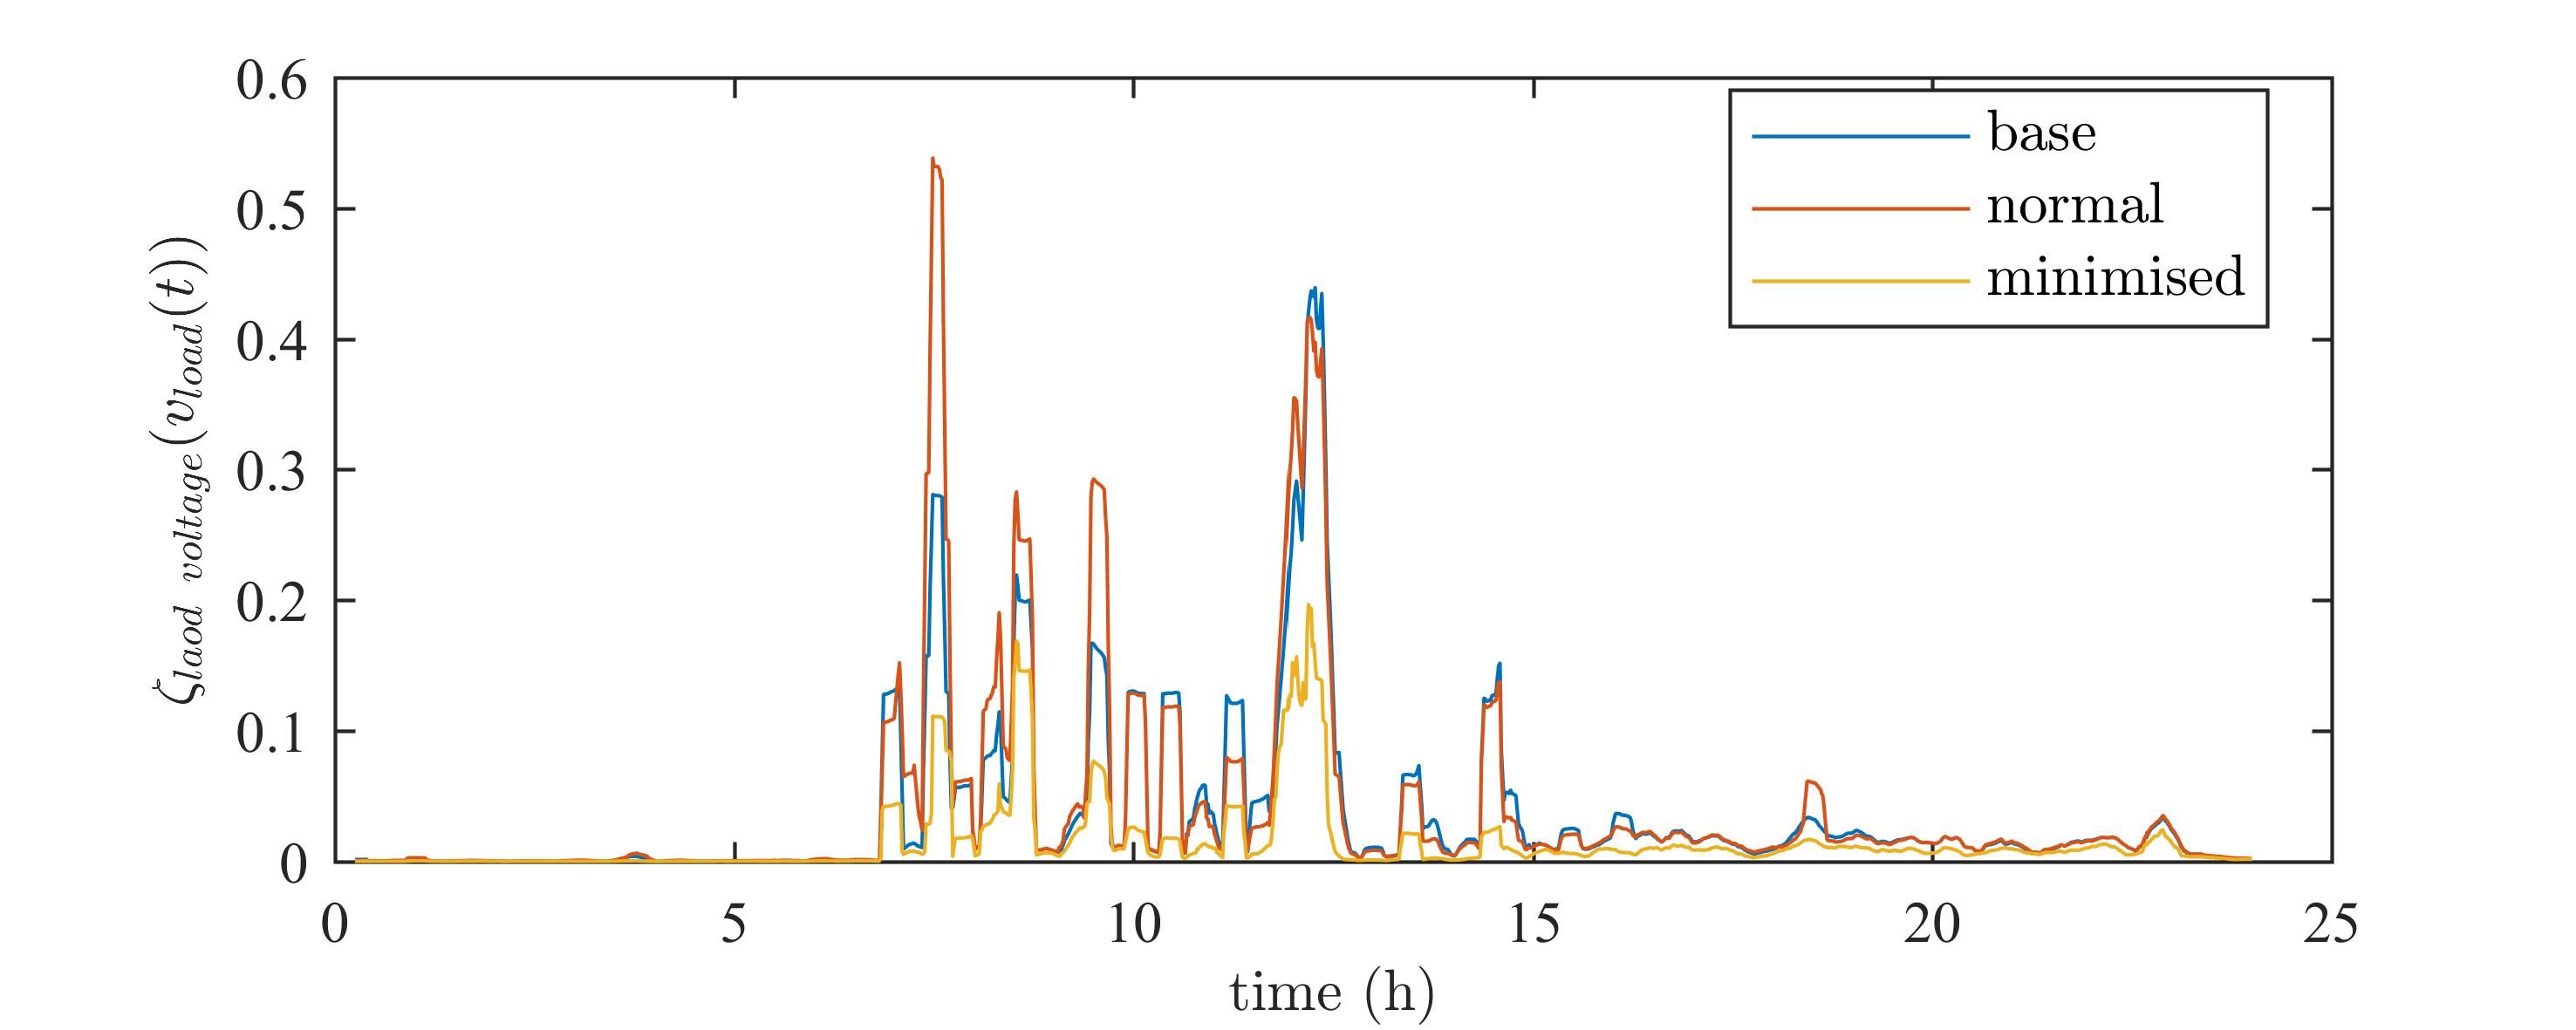
\includegraphics{_chapter1/fig/results/ts-all-voltages}%
		\label{ch1:subfig:ts-all-voltages-cost}%
	}
\caption{Voltage level improvements at all buses in the entire distribution network due to the ESMU schedule adjustment.}
\label{ch1:fig:ts-all-voltages}
\end{figure}


\subsection{Difference Analysis}
\label{ch1:subsec:difference-analysis}


\subsection{Probability Density Analysis}
\label{ch1:subsec:probability-density-analysis}
